\chapter{Généralités}
\thispagestyle{fancy}
\section{Introduction}
Nous présentons dans ce chapitre les principaux concepts liés au \emph{\gls{Fog Computing}}. Nous commençons d'abord par introduire l'Internet des objets et leur relation au Fog Computing. Puis, nous expliquons les techniques de migration de conteneurs entre les nœuds Fog. Enfin, nous terminons ce chapitre par une taxonomie des travaux similaires axés sur la gestion de ressources des nœuds Fog, ainsi que les différents défis rencontrés. 
\section{Internet des objets (IoT)}
\subsection{Définition}
Le terme Internet des objets (Internet of Things ou \emph{\gls{IoT}}) décrit le réseau d'appareils physiques - souvent hétérogène - interconnectés, et dont le rôle principal est la récolte et l'échange d'information, ainsi que l'interaction avec l'environnement extérieur \cite{patel2016}. Cette infrastructure est dite intelligente, dotée de la capacité de s'auto-organiser, partager l'information de manière optimale et de réagir aux changements environnementaux \cite{madakam2015}.\par
Les objets dans ce type de réseau sont de capacité limitée, que ce soit en puissance de calcul ou en consommation d'énergie. Ce sont majoritairement des objets électroniques quotidiens (à l'exemple de smartphones, véhicules ou équipements ménagers), chacun avec sa propre identité pour communiquer avec le reste des objets et synchroniser les efforts de réponses aux différentes situations externes auxquelles ils sont exposés.

\subsection{Histoire et Évolution}
L'idée d'interconnecter des dispositifs électroniques moyennant un réseau informatique est apparue dans les années 80s, à l'Université de Carnegie Melon, où on avait relié un distributeur de boissons fraîches à un ordinateur de monitorage. Ce qui a permis aux programmeurs de consulter la disponibilité des boissons à distance et d'éviter les trajets inutiles \cite{madakam2015}.\par
Cependant, le premier à avoir introduit ce concept est Kevin Ashton en 1999, qui travaillait dans l'optimisation de chaîne de production chez Procter \& Gamble. Ashton avait constaté qu'en 1999, 50 petabytes d'information étaient créés par des êtres humains. D'où, il a dévelopé l'idée de décharger l'homme de cette tâche fastidieuse de récolte d'information et ce, lors d'une présentation portant le nom de la technologie (Internet of Things). Il propose plutôt d'exploiter la masse d'engins et de capteurs disponibles et déjà déployés à ce moment là \cite{ashton2009}.\par
Cette infrastructure n'a été adoptée en industrie qu'en fin de l'année 2000s. Depuis, les constructeurs du domaine de téléinformatique concentrent leurs efforts sur la production de capteurs et d'appareils IoT avec différentes fonctionnalités dans le but de combler les besoins des diverses industries, allant de l'agriculture et domaine médical jusqu'à l'industrie militaire.

\subsection{Architecture}
L'architecture d'un réseau IoT se décompose en 4 couches flexibles. Chaque couche est constituée de plusieurs technologies et standards \cite{patel2016}. Cet aspect modulaire permet une meilleure scalabilité de l'infrastructure et une meilleure adaptation aux besoins émergeants. Les couches de ce modèle sont comme suit:
\begin{enumerate}
  \item \emph{La couche de capteurs et d'objets intelligents:} Elle est formée d'objets connectés munis de capteurs et/ou d'actionneurs. C'est la couche la plus proche de l'environnement physique, celle-ci transforme les événements générés par ce dernier en un flux d'information à temps réel, et se charge de leur transmission. Les capteurs ont différentes spécifications, comme la mesure de la température, ou la pression, la capture de mouvement …, et sont connectés soit à des passerelles à l'aide de réseaux filaires (Ethernet) ou non (Wi-Fi, Bluetooth, RFID …), soit directement à la couche applicative. Un exemple de ce type de technologie est les WSNs, caractérisés par leur basse consommation d'énergie et grande zone de couverture.
  \item \emph{La couche réseau et passerelles:} Cette couche garantit la transmission de la masse d'information générée par la couche précédente, tout en respectant la qualité de service exigée par les applications servies. Plusieurs infrastructures et protocoles de communication ont été mis en place dans le but d'optimiser l'acheminement et traitement d'information, comme le concept de Fog Computing qu'on détaillera par la suite.
  \item \emph{La couche de gestion:} Le rôle de cette couche est de filtrer et organiser les informations, en fournissant une couche d'abstraction à l'application. Elle s'occupe de la gestion de priorité, et l'analyse de la pertinence des données. C'est aussi à ce niveau que les politiques d'anonymisation et sécurisation de données sont implémentées.
  \item \emph{La couche d'application:} Elle est située majoritairement dans des clouds ou data-centers. Les applications couvrent des domaines différents comme l'agriculture et la gestion de villes intelligentes, et d'autres plus critiques, comme le domaine de la santé ou le domaine militaire. Toutefois, depuis quelques années, les efforts de recherche visent à rapprocher ces applications de la première couche du modèle, pour des motifs que nous expliquerons dans la section dédiée au Fog Computing. 
\end{enumerate}

\subsection{Quelques domaines d'application}
L'installation d'objets intelligents s'est démocratisée depuis quelques années. On les retrouve dans les environnements suivants:
\begin{itemize}
  \item Les systèmes de sécurité et surveillance, où des caméras et capteurs de mouvements permettent de détecter et identifier toute activité suspecte.
  \item Les maisons intelligentes: ce qui décrit la connectivité des objets dans un domicile, tous œuvrent pour fournir de meilleures conditions de vie, et ceci en assurant: la régulation de températures, l'optimisation de consommation d'énergie, la détection d'incendie et le filtrage de l'air.
  \item Les systèmes de voitures autonomes dans lesquels les véhicules utilisant la voie publique peuvent s'échanger des informations, parfois critiques, et alerter les conducteurs de tout danger imminent. Ils peuvent aussi, en se basant sur les informations de géolocalisation fournies par les autres usagers, produire des recommandations de destination tout en évitant les points de congestion de la circulation routière.
  \item Les dispositifs permettant la surveillance médicale de personnes incapacités, et ainsi la prise de dispositions nécessaires dans les moments d'urgence.
\end{itemize}

\subsection{Problèmes et difficultés}
Le provisionnement en énergie est devenu une des préoccupations de la société actuelle. On cherche à optimiser l'utilisation de ressources énergétiques, soit pour étendre l'autonomie des objets et capteurs mobiles, ou bien pour réduire les frais d'approvisionnement en électricité. Des algorithmes de gestion et allocation des ressources ont été proposés pour minimiser cette consommation, mais les recherches sur ce sujet sont toujours actives.\par
Avec la croissance du nombre d'objets connectés, les attaques cybercriminelles deviennent excentriques. Ce réseau peut être vulnérable contre l'injection de données erronées qui peuvent influencer des prises de décision parfois critiques. Les nœuds intercommunicants disposent de ressources limitées, et ainsi, ils peuvent être sujets à des attaques de déni de service (\emph{DDOS}). La grande quantité de données produite doit être protégée tout au long du circuit liant les couches présentées précédemment. Un travail de supervision doit être mené dans le but de garantir la confidentialité des données récoltées, et empêcher les pratiques abusives comme la vente de données d'utilisateurs \cite{COLAKOVIC201817}.\par
De plus, certaines applications demandent une certaine réactivité et une grande vitesse de réponse pour accomplir des missions critiques comme pour la conduite de véhicules automobiles ou la surveillance médicale. Ces exigences sont souvent restreintes par d'autres contraintes comme la mobilité des objets connectés ou la congestion dans le réseau de communication.
%------------------------------------------------------------
\section{Fog Computing}

\subsection{Histoire et évolution}
Malgré les avantages considérables que procure le \emph{\gls{Cloud Computing}} en termes de performance, d'accessibilité et de scalabilité, Ce dernier se heurte néanmoins à quelques limites face à l'expansion de l'Internet des objets (IoT), ce qui impose donc une réévaluation de ce paradigme. \par 
En effet, l'accélération de la croissance du nombre d'appareils connectés à Internet ainsi que l'énorme quantité de données générées par ces derniers ont démontré une certaine limitation du paradigme Cloud. Le problème le plus apparent est le problème de \emph{\gls{latence}}, en vue donc de la croissance de la quantité de données générées par les différents objets connectés et la dépendance de ces derniers visés à vis du Cloud pour le traitement de ces données, ceci risque de provoquer une réduction considérable des performances du réseau, ce qui engendrerait une augmentation des délais de transfert et donc une diminution des performances de traitement. Ce qui peut être critique au niveau de certaines applications notamment les applications qui requièrent des traitements en temps réel.\\
D'autres problèmes peuvent être cités également, comme le problème de congestion ou encore le problème de connaissance de localisation. \par
C'est pour répondre donc à ces problèmes que le Fog Computing a été proposée comme une extension du paradigme Cloud en 2012, et qui a vu par la suite la création d'un consortium dédié qu'est l'\textbf{OpenFog Consortium} afin de faciliter l'interopérabilité des différentes solutions technologiques.

\subsection{Définition et concept}
Selon CISCO \cite{bonomi2012}, le terme \emph{Fog computing} désigne : \og{}une plate-forme hautement virtualisée qui fournit des services de calcul, de stockage et de mise en réseau entre les appareils finaux et les centres de données de Cloud Computing traditionnels, située généralement, mais pas exclusivement, à la périphérie du réseau\fg{}.\par
L'\emph{OpenFog Consortium} \cite{OpenFog2017} le définit aussi comme étant : \og{} Une architecture horizontale au niveau du système qui distribue des fonctions de calcul, de stockage, de contrôle et de mise en réseau plus proches des utilisateurs le long du continuum Cloud-objet\fg{}.\par
Le terme réfère aussi à une infrastructure matérielle et applicative distribuée qui vise à stocker et à traiter les données issues des différents appareils connectés afin de se substituer au Cloud pour certains traitements.\par
La principale idée du Fog Computing est l'instrumentalisation des différents équipements qui constitue les noeuds du réseau (routeurs, commutateurs, passerelles, etc.) comme étant un centre de traitement et de stockage de donnés distribué qui est à la fois intermédiaire au Cloud et en même temps proche des extrémités du réseau.
En créant donc une couche auprès de la production des données, ceci entraîne une réduction des transferts entrant et sortant du Cloud et donc une réduction de la latence, et par conséquent du temps des différents traitements et services.

\subsection{Architecture}
La plupart des recherches qui s'orientent vers la définition d'un modèle architectural semblent se diriger vers un même modèle, à savoir un modèle en 3 couches \cite{de2019}.\\
Les couches de ce modèle sont présentées comme suit :
\begin{description}
  \item[Couche IoT :] cette couche désigne l'ensemble des appareils se trouvant à l'extrémité du réseau, elle est composée essentiellement d'appareils IoT tels que des véhicules intelligents, des smartphones, des drones militaires, des capteurs sensoriels, etc. Le rôle de ces derniers étant la collecte et la transmission des données vers la couche supérieure pour stockage ou traitement.
  \item[Couche de Fog :] cette couche constitue le point central du paradigme Fog, elle est constituée d'un ensemble de nœuds Fog, qui selon le OpenFog Consortium, ce dernier se définit comme 
  \og{}un élément physique ou logique qui implémente les services informatiques Fog\fg\cite{de2019}.\par
  L'ensemble des nœuds constitue un centre de traitement et de stockage distribué connecté à la fois à la couche inférieure et celle supérieure à travers des nœuds passerelles, permettant ainsi de bénéficier des différents services fournis par la couche supérieure qu'est le Cloud par exemple le stockage, tout en fournissant des informations contextuelles aux utilisateurs au niveau de la couche inférieure.
  \item[Couche Cloud :] cette couche représente une infrastructure Cloud centralisée. Elle est composée de ressources matérielles élevées et fournit différents services, ayant comme différences avec une architecture en Cloud classique, certains traitements et services qui sont déchargés de la couche Cloud au profit de la couche Fog afin d'équilibrer la charge de travail et d'augmenter l'efficacité et la fiabilité.] 
\end{description}

\begin{figure}[H]
  \centering
  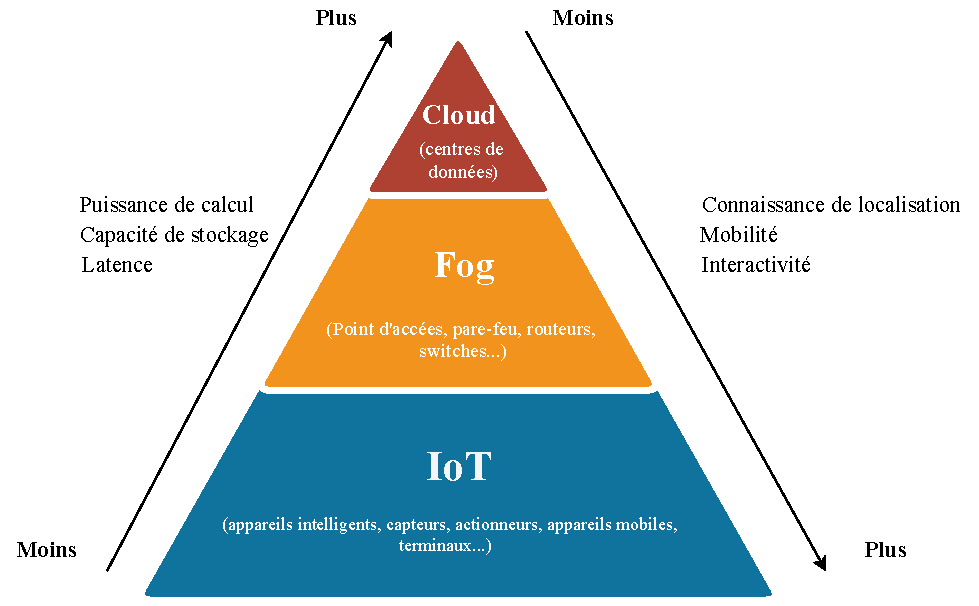
\includegraphics[scale=0.8]{ArchitectureFog.pdf}
  \caption{Architecture du Fog Computing}
  \label{fig:architectureFog}
\end{figure}

%\subsection{Avantages}
%Le Fog computing présente de nombreux avantages qu'il convient de souligner, Ils sont généralement résumés sous le sigle SCALE pour :
%\begin{itemize}
%  \item \emph{Sécurité :} Dans ce paradigme, la sécurité est prise en considération lors de l'élaboration de l'architecture plutôt qu'une partie optionnelle.
%  \item \emph{Cognition :} vient du fait que l'infrastructure Fog est consciente des besoins et exigences des utilisateurs. Elle distribue ainsi plus finement les ressources en fonction de chaque utilisateur contrairement au Cloud.
%  \item \emph{Agilité :} Ce qui désigne la capacité d'adaptation rapide à l'innovation.
%  \item \emph{Latence :} En raison de sa proximité avec les utilisateurs finaux, le Fog a la capacité de supporter des applications qui nécessitent des latences courtes et stables, évitant ainsi les problèmes résultant des systèmes centralisés.
%  \item \emph{Efficacité :} vient du fait que cette vision étant les capacités du Cloud en intégrant
%  les différents nœuds qui composent le réseau à l'infrastructure de traitement et de stockage, augmentant ainsi la capacité ainsi que l'efficacité globale du système.
%\end{itemize}

%\subsection{Défis et verrous scientifiques}
%Bien que le Fog Computing ait apporté des avantages considérables, ce paradigme reste relativement récent et nécessite  d'investiguer certains défis, par exemple :
%\begin{itemize}
%  \item \emph{Gestion de l'énergie:} Les infrastructures de Fog comprennent généralement un grand nombre de nœuds géo-distribués. La consommation énergétique est donc plus élevée en comparaison avec celle du Cloud. De grands efforts de recherche sont alors nécessaires pour développer des solutions efficaces afin de minimiser l'empreinte énergétique, par exemple, des algorithmes de traitement et des protocoles de communication moins coûteux en énergie sont à développer.
%  \item \emph{Hétérogénéité:} En plus de l'hétérogénéité trouvée dans les environnements IoT, aux nivaux des types d'objets connectés, des données, des technologies de communications et des performances. Ce problème est également présent dans les infrastructures Fog en raison de la diversité des équipements qui constituent les nœuds Fog. La gestion de l'hétérogénéité dans un environnement de Fog et d'IoT représente un défi important.
%  \item \emph{Gestion et provision de ressources:} Les noeuds Fog sont généralement des équipements à capacité limités, il est par conséquent indispensable de disposer de solution efficace en termes de gestion de ressource, par exemple l'ordonnancement des différentes applications.
%\end{itemize}
%------------------------------------------------------------
\section{Migration dans les environnements Fog Computing}

\subsection{Définitions et concepts}
La \emph{\gls{virtualisation}} introduit une couche d'abstraction logicielle entre le matériel et le système d'exploitation ou les applications qui s'exécutent dessus. En séparant les ressources logiques des ressources physiques sous-adjacentes, la virtualisation permet l'affectation flexible de charges de travail entre les machines physiques.
La \emph{\gls{migration}} d'instance virtuelle (\emph{\gls{machine virtuelle}} ou \emph{\gls{conteneur}}) est considérée comme le processus de copie et déplacement de l'état de cette dernière d'un hôte physique à un autre \cite{boutaba2013}.\par
\subsection{Migration VMs-Conteneurs}
La migration d'instance virtuelle joue un rôle essentiel dans les environnements Fog étant donné qu'elle permet de garantir la continuité des services, quels que soient les besoins en mobilité exprimés par les objets connectés à cet environnement.
Il existe deux grandes techniques de virtualisation logicielle exploitées dans les architectures orientées services: les machines virtuelles et les conteneurs. Leurs principales différences résident dans leur évolutivité et leur portabilité \cite{redhat} (voir Figure \ref{fig:vmvsconteneur}).\par
Dans le cas général, le volume d'un conteneur se compte en mégaoctets. Il ne comporte rien de plus gros qu'une application et ses fichiers qu'elle en dépend. Ce sont des paquets à monofonctionnalité, effectuant des tâches spécifiques (appelées microservices) \cite{redhat}. C'est une méthode de virtualisation au niveau du système d'exploitation(Software Virtualization) qui vise à exécuter plusieurs systèmes totalement isolés (conteneurs) sur un seul hôte de contrôle (un simple système d'exploitation). Les conteneurs partagent le noyau avec l'hôte et fournissent un environnement indépendant qui possède son propre CPU, mémoire, bloc d'E/S, réseau et le mécanisme de contrôle des ressources.\par
D'autre part, une machine virtuelle est plus volumineuse (plusieurs gigaoctets), comporte son propre système d'exploitation y compris son noyau. Elle permet l'exécution simultanée de plusieurs fonctions gourmandes en ressources \cite{microsoft2019}. L'ensemble de machines virtuelles sur une même machine sont gérées par un hyperviseur, qui permet leur isolation en s'exécutant sur des hôtes physiques et il est également responsable de la coexistence de différents noyaux des machines virtuelles au sein d'une même machine physique.\par
Donc la différence principale est que les conteneurs permettent de virtualiser un système d'exploitation afin que plusieurs charges de travail s'exécutent sur un système d'exploitation unique (on peut prendre l'exemple d'une base de données MySQL qu'on aura comme copie individuelle dans une machine virtuelle, mais avec l'utilisation des conteneurs on aura la possibilité d'avoir plusieurs copies des services de ce dernier).\par
Les conteneurs partagent en pratique le même noyau du système d'exploitation hôte contrairement aux technologies de machines virtuelles où le matériel est virtualisé pour exécuter plusieurs instances de système d'exploitation. Cela permet de lancer un nombre beaucoup plus important de conteneurs que de machines virtuelles sur le même matériel, et ainsi fournir une haute disponibilité capable de satisfaire la demande imposée par les réseaux de nouvelle génération telle que la 5G. Des exemples de systèmes à base de conteneurs sont Docker, OpenVZ, LXC et LXD. 
\begin{figure}[H]
\centering
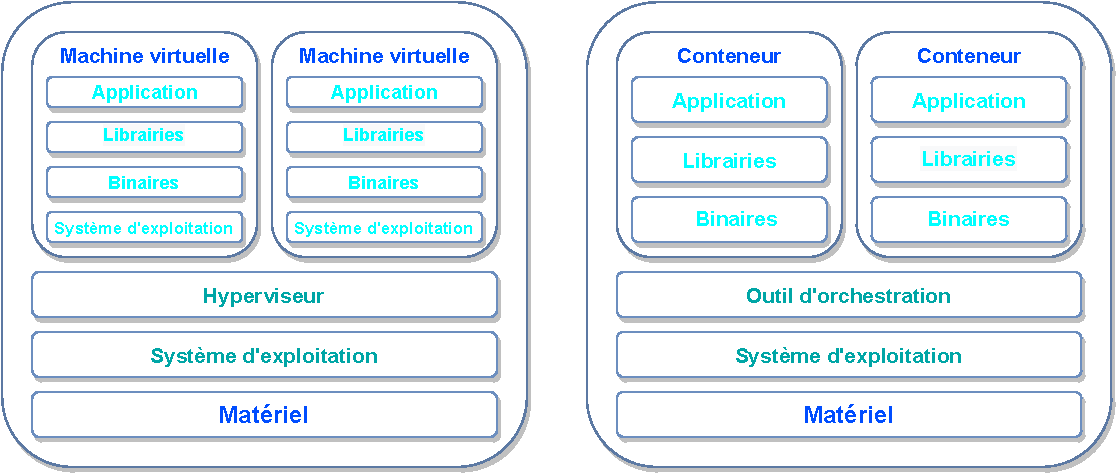
\includegraphics[scale=0.8]{vm-container.pdf}
\caption{Architecture de machine virtuelle, et de conteneur \cite{alibabacloud}}
\label{fig:vmvsconteneur}
\end{figure}

\subsection{Avantages et inconvénients}
\subsubsection{Avantages de la virtualisation et de la migration}
La dynamicité de ce mécanisme de migration confère une flexibilité dans la distribution et organisation des tâches de travail sur l'ensemble des ressources matérielles. Cela permet de répondre efficacement aux fluctuations des charges en mobilisant les conteneurs et machines virtuelles selon le besoin. Deux utilisations sont envisageables comme suit \cite{boutaba2013}.\par
D'une part, la migration permet de consolider les serveurs, en regroupant les instances virtuelles sur un nombre réduit de machines. Cette utilisation est particulièrement efficace dans le scénario de charge réduite et considérablement inférieure à la capacité de traitement totale disponible. Ceci afin de permettre la mise en veille ou la suspension des machines non exploitées et en l'occurrence réduire la consommation énergétique et ainsi les coûts engendrés.\par
D'une autre part, et dans les conditions opposées à celles susmentionnées, c'est-à-dire dans un environnement qui exige de grandes capacités de traitement, la précédente technique cause une surcharge sur les machines exploitées et par la suite une dégradation du temps de réponse et réduction du temps de disponibilité du service. Pour pallier ces contrecoups, la migration de machines virtuelles et de conteneurs est employée pour instaurer et assurer une uniformité dans la distribution des tâches entre les ressources physiques disponibles.\par
Ainsi, trouver un compromis optimal entre la consolidation de serveurs et l'équilibrage de charge est essentiel pour parvenir à une utilisation efficace des ressources dans les centres de données virtualisés.\par
Le mécanisme de migration permet aussi d'améliorer la localisation des données dans un réseau notamment dans des environnements Fog ou pour servir des applications hautement mobiles, résultant en une meilleure exploitation de la bande passante et la réduction du délai de communication.\par
De plus, ce mécanisme permet de conserver la continuité du service lors des maintenances routinières ou de pannes matérielles, et de minimiser les conséquences des erreurs humaines ou catastrophes naturelles en transférant les services critiques de façon réactive.

\subsubsection{Inconvénients}
Malgré ces avantages, la migration de VM (machine virtuelle) ou de contenaire présente quelques désavantages, parmi lesquels on cite:
\begin{itemize}
  \item Le coût en consommation de ressources engendré par l'opération de migration, en bande passante, temps de calcul CPU et disque.
  \item La discontinuité du service malgré l'existence de techniques qui réduisent ce dernier, mais qui reste toutefois inévitable.
  \item Dans le cloud public actuel, les machines virtuelles sont installées sur les mêmes machines physiques. Certaines des machines virtuelles travaillant dans le même sous-réseau ou serveur physique peuvent collaborer afin de satisfaire un service. La collaboration et les connexions entre VM via le réseau ainsi que le partage de ressources physiques augmentent le risque de vulnérabilité de sécurité, et de contamination par des VM malicieuses \cite{chandrakala2018}.
\end{itemize}

\subsection{Techniques de migration}
Nous nous intéresserons dans cette partie aux techniques de migration de conteneurs. Cependant, les idées de base s'appliquent également à la migration des applications et à la migration des VMs. La migration a été rendue possible grâce à l'introduction des technologies de la virtualisation, ces derniers ont permis la séparation entre la charge de travail (workload) et le matériel du serveur (hardware).\par
Le temps d'arrêt (Downtime) est la période pendant laquelle les services fournis par la VM ou le conteneur migrant ne sont pas disponibles ou ne répondent plus aux demandes des utilisateurs.\par
Le temps total de migration est la durée de temps qui sépare le lancement du processus de migration et l'instant de mise à disposition de l'instance du serveur de destination. Ce qui correspond à la somme du temps d'arrêt et temps nécessaire pour la copie du disque et la mémoire système.\par
Nous distinguons deux types de migrations \cite{puliafito2019}:
\begin{description}
  \item[La migration sans état:] Le conteneur est redémarré de nouveau sur le nouvel hôte ce qui implique la perte de l'ancien état d'exécution. Elle se compose de deux étapes:
  \begin{enumerate}
    \item Lancement du nouveau conteneur sur la machine de destination.
    \item L'arrêt et suppression de l'ancien conteneur de la machine source.
  \end{enumerate}
  \item[La migration avec état:] Dans ce type de migration, on conserve les données et contextes d'exécution lors du transfert, et deux techniques sont utilisées:
    \begin{enumerate}
      \item \emph{La migration à froid}: Dans cette approche l'instance est suspendue au lieu d'être complètement arrêté comme dans une migration froide. L'environnement virtuel est déplacé vers un autre serveur et le système d'exploitation est repris à destination. L'état des applications dans le système d'exploitation invité peut être conservé pendant la migration (stateful-state). La durée de l'indisponibilité est égale à la durée totale de migration (voir Figure \ref{fig:migration_a_froid}). Par contre, les pages mémoires ne sont transférées qu'une seule fois, ce qui réduit le temps de transfert et la quantité de données échangées.
      \begin{figure}[H]
      \centering
      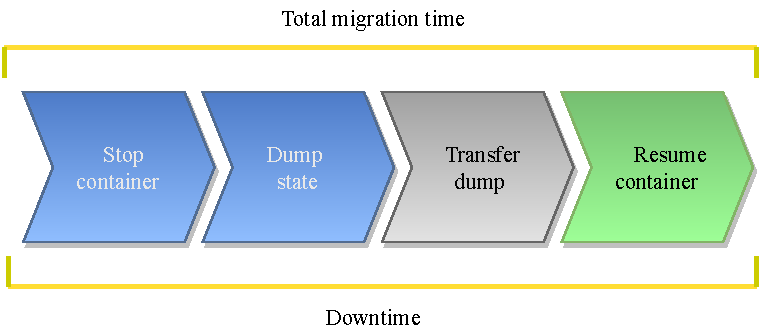
\includegraphics[scale=1]{migration_a_froid.pdf}
      \caption{La migration à froid \cite{puliafito2019}}
      \label{fig:migration_a_froid}
      \end{figure}
      \item \emph{La migration à chaud}: Contrairement à la migration à froid, les pages de mémoire de l'instance seront conservées et copiées vers l'hôte de destination pendant son exécution. Après quoi il reprend son exécution sur l'hôte de destination. On distingue trois sous-catégories de migration à chaud:
        \begin{enumerate}
          \item La migration avec pré-copie.
          \item La migration avec post-copie.
          \item La migration hybride.
        \end{enumerate}
      \end{enumerate}
\end{description}
\textbf{La migration avec pré-copie (méthode itérative)}: Dans ce cas, toutes les pages sont transférées au serveur de destination avant de geler le container. Mais quand les processus continuent leur exécution normale, les pages peuvent être modifiées et les pages transférées peuvent devenir obsolètes. C'est pourquoi les pages doivent être transférées itérativement. Sur la première étape, toutes les pages sont marquées d'un drapeau propre (clean flag) et transférées sur le serveur de destination [46]. Certaines pages peuvent être modifiées pendant ce processus, et l'indicateur propre sera supprimé dans ce cas. Sur la deuxième étape, seules les pages modifiées sont transférées vers le serveur de destination (voir Figure \ref{fig:migration_avec_precopie1}). La figure \ref{fig:migration_avec_precopie2} montre le séquencement des opérations de cette migration.\par
\begin{figure}[H]
\centering
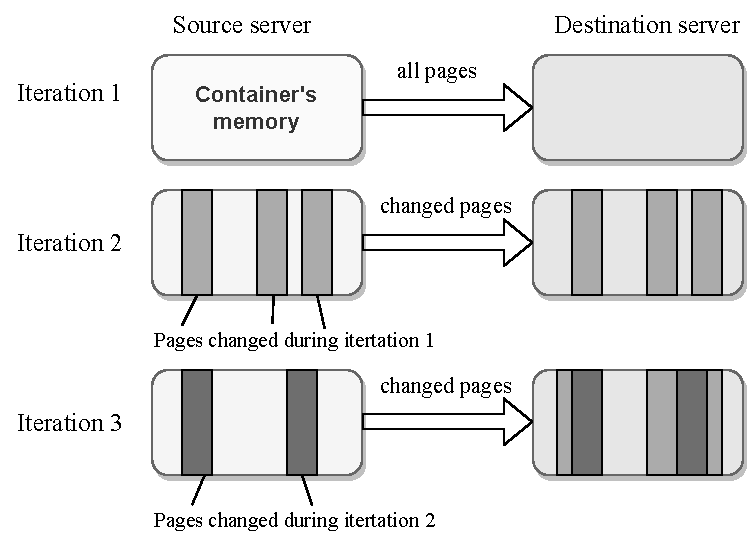
\includegraphics[scale=0.9]{iterative_migration.pdf}
\caption{Itérations de la migration avec pré-copie \cite{mirkin2008}}
\label{fig:migration_avec_precopie1}
\end{figure}
\begin{figure}[H]
\centering
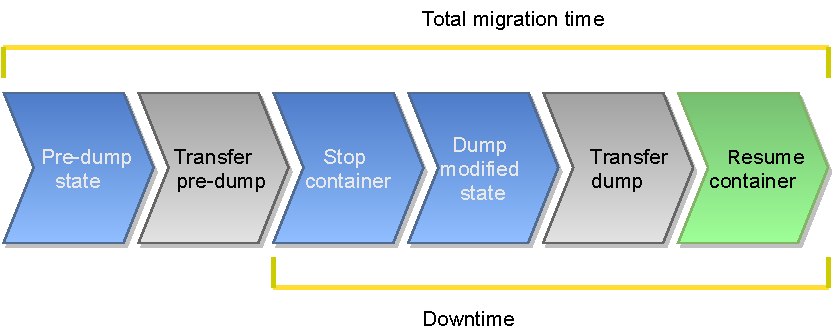
\includegraphics[scale=1]{migration_avec_precopie.pdf}
\caption{La migration avec pré-copie \cite{puliafito2019}}
\label{fig:migration_avec_precopie2}
\end{figure}
\textbf{La migration avec post-copie (fainéante)}: Par opposition à la technique précédente, toutes les pages mémoire allouées par les processus sont marquées d'un drapeau spécial, qui est effacé si une page est modifiée. Après cela, un conteneur peut être gelé et son état peut être sauvegardé, mais dans ce cas, seules les pages sans cet indicateur sont stockées. Cela permet de réduire la taille d'un fichier de vidage (dump). Puis au besoin, la machine destination génère des demandes de pages défectueuses (page-in swap), auxquelles la machine source répond en envoyant ces pages (à l'aide du daemon “page-out”), puis ces pages sont chargées en mémoire sur le serveur de destination (voir Figure \ref{fig:migration_avec_postcopie1}). C'est pour cette raison qu'elle est appelée migration fainéante. La figure \ref{fig:migration_avec_postcopie2} donne le schéma global de cette migration.\par
\begin{figure}[H]
\centering
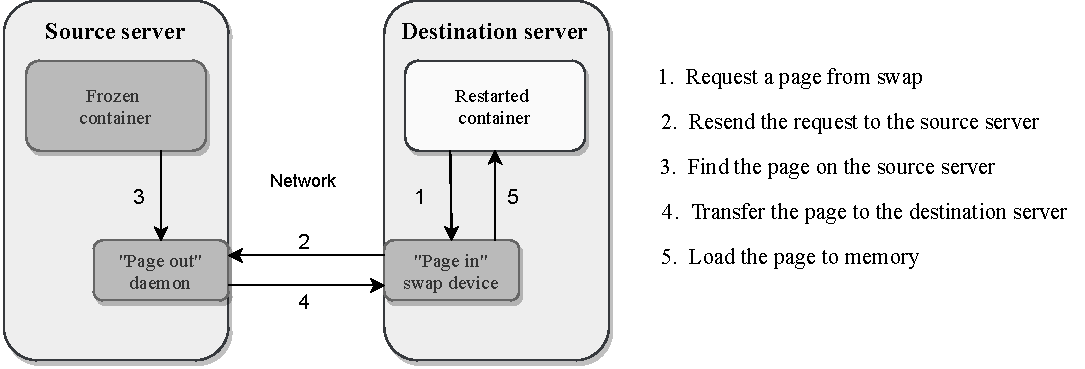
\includegraphics[scale=0.9]{lazy_migration.pdf}
\caption{Envoi des pages défectueuses \cite{mirkin2008}}
\label{fig:migration_avec_postcopie1}
\end{figure}
\begin{figure}[H]
\centering
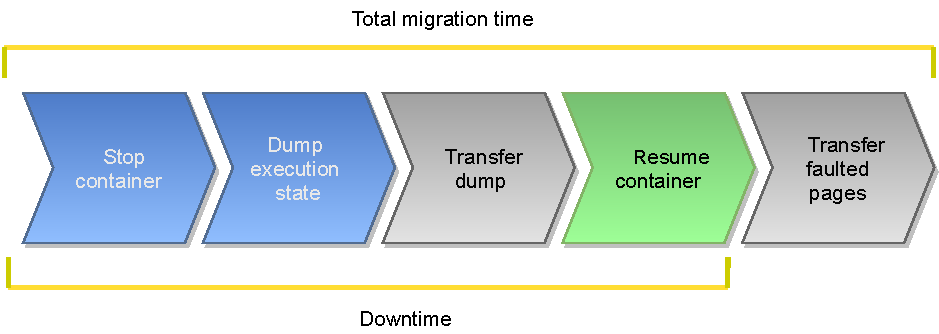
\includegraphics[scale=1]{migration_avec_postcopie.pdf}
\caption{La migration avec post-copie \cite{puliafito2019}}
\label{fig:migration_avec_postcopie2}
\end{figure}
\textbf{La migration hybride}: Les premières étapes coïncident avec celles de la migration avec pré-copie, une seule phase de pré-copie est effectuée avant la phase de post-copie,de cette manière l'hôte cible dispose déjà de toute la mémoire, seules les pages sales devront être transférées en post-copie. Une fois la mémoire copiée, le conteneur source est arrêté, et le conteneur destination est lancé sur l'hôte cible et la phase de post-copie commence \cite{wikimigration} (voir Figure \ref{fig:migration_hybride}).
\begin{figure}[H]
\centering
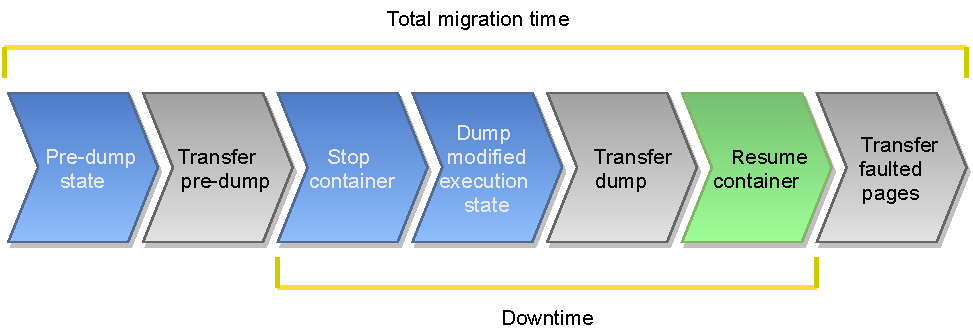
\includegraphics[scale=1]{migration-hybride.pdf}
\caption{La migration hybride \cite{puliafito2019}}
\label{fig:migration_hybride}
\end{figure}

\subsection{Taxonomie, Travaux réalisés}
Les travaux réalisés dans le domaine de virtualisation et migration de ressources virtuelles ont été classifiés selon la littérature en trois catégories selon l'objectif à optimiser \cite{rejiba2019}.
\begin{itemize}
  \item \emph{Optimisation du coût de la migration} : Visant soit à réduire les migrations coûteuses ou à trouver des compromis de coût de migration. Les processus de décision markovien constituent l'une des approches les plus utilisées pour modéliser le compromis de migration. Plus récemment, les efforts se sont progressivement déplacés vers la résolution du problème MDP en utilisant des approches apprentissage approfondi, qui ne nécessitent pas de connaissances préalables sur la dynamique de l'environnement MDP.
  \item \emph{Optimisation du temps de migration} : Les optimisations de migration focalisées sur l'axe du temps peuvent être divisées en optimisations proposées au niveau de la technologie de virtualisation et optimisations résultant de la prise d'actions proactives.
  \item \emph{Optimisation du taux d'erreur de la migration} : Les recherches sur ce sujet viennent exclusivement du domaine du cloud véhiculaire, à cause de la dynamicité le caractérisant, et qui peut potentiellement troubler le taux de succès de la migration. Ici, des techniques d'intelligence artificielle sont employées pour prédire la durée de disponibilité d'un véhicule dans une zone de couverture. Des protocoles de communication plus adaptés (comme le V2V) ont été aussi proposés.
\end{itemize}

%------------------------------------------------------------
\section{Gestion des ressources dans les environnements Fog Computing}
Contrairement au \emph{Cloud}, les ressources du \emph{Fog} sont : 
\begin{itemize}
  \item limitées en termes de performance et d'énergie - La plupart des noeuds \emph{Fog} possèdent généralement une  puissance de calcul ainsi que des ressources énergétiques limitées, dues principalement au fait que ces derniers sont constitués généralement des équipements d'interconnexion qui composent le réseau.
  \item hétérogènes - aussi bien sur le plan matériel, tel que différentes architectures de processeur, que sur le plan logiciel tel que différents systèmes d'exploitation.
  \item sujets à des défaillances - Les nœuds \emph{Fog} sont très susceptibles de subir des anomalies tels que des pannes de courant ou des défauts de capacité qui empêchent l'exécution des applications affectée à eux.
\end{itemize}
Dans de telles conditions, une gestion optimale des ressources est indispensable pour faire du \emph{Fog computing} une réalité. Ce qui fait de la gestion de ressource l'un des principaux défis du paradigme.

\subsection{Définition}
Selon \cite{red2020}, la gestion de ressources dans les environnements \emph{Fog} désigne \og{}les opérations administratives telles que le déploiement, la virtualisation et la surveillance des nœuds \emph{Fog} qui favorise les services d'infrastructure et de plate-forme basés sur le \emph{Fog}. De plus, la gestion des ressources du \emph{Fog} réalise l'équilibrage de charge, l'approvisionnement dynamique et la mise à l'échelle automatique pour assurer disponibilité du service et multi-location\fg{}.

\subsection{Dimensions du problème}
Le problème de la gestion des ressources dans les environnements \emph{Fog} est un problème complexe. Il ne peut donc pas être considéré comme étant un seul problème, mais plusieurs problèmes suivant plusieurs aspects \cite{mos2019}. Le problème peut être vu suivant  6 axes principaux que sont : le placement d'application, l'ordonnancement des tâches, le déchargement des tâches, l'équilibrage de charges, l'allocation de ressources ainsi que l'approvisionnement en ressources.
\begin{figure}[H]
  \centering
  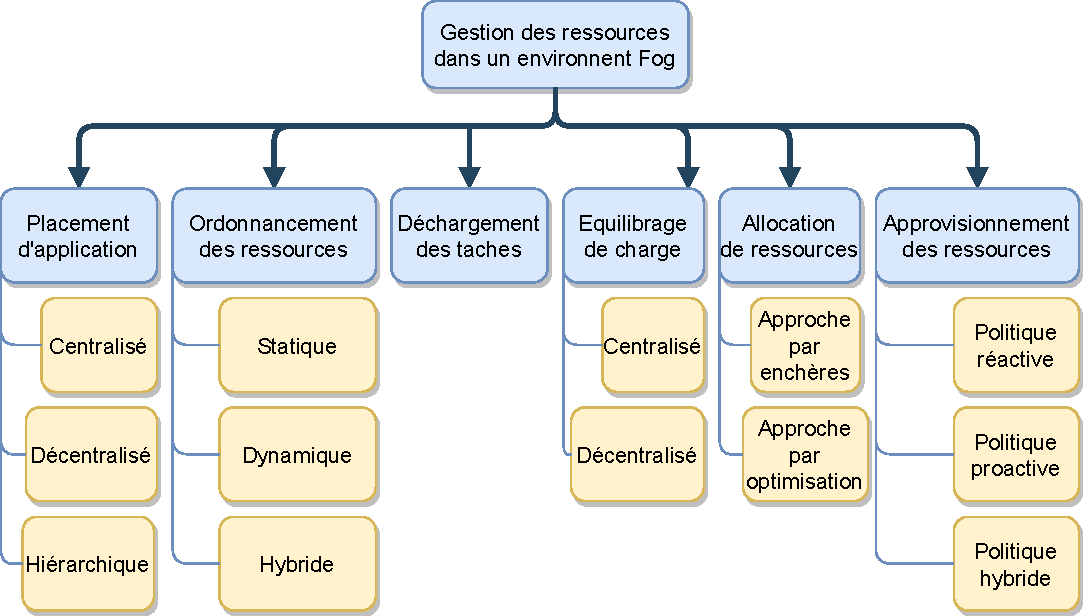
\includegraphics[scale=0.9]{organigrame_gestion_de_ressources.pdf}
  \caption{Organigramme qui illustre les domaines de gestion de ressource ainsi que leurs approches}
  \label{fig:organigrame_de_gestion_de_ressources}
\end{figure}

\subsubsection{Placement d'application}
Le problème de placement d'application désigne le problème de trouver une manière d'associer un service \emph{IoT} aux nœuds \emph{Fog} répondant aux exigences de la Qualité de service (QdS), tout en essayant de maximiser l'utilisation des différents nœuds .\\
D'une manière plus formelle soit $S$ un service \emph{IoT} avec des exigences de QdS $Q$, et soit $N$ l'ensemble des noeuds \emph{Fog}.\\
Une solution au problème de placement d'application consiste à associer au service $S$ un nœud \emph{Fog} $N_{i}$ de $N$ satisfaisant les exigences de QdS $Q$, tout en optimisant un ensemble de fonctions objectives $O$.\\
Il convient de préciser que les solutions peuvent être des relations multivaluées \emph{i.e.} un service \emph{IoT} peut être placé sur un ou plusieurs nœuds et réciproquement, un nœud peut héberger un ou plusieurs services.\par
Les approches basées sur la gestion de courtier “Broker” peuvent être organisées en 3 catégories que sont : l'approche centralisée, décentralisée et hiérarchique.
\begin{itemize}
  \item Dans l'approche centralisée, le broker nécessite d'avoir une vision globale de tout l'environnement \emph{Fog} afin de prendre des décisions d'optimisation pour l'ensemble du système. Cette approche ne garantit pas une optimisation efficace due à la difficulté d'obtenir toutes les informations de toutes les entités du \emph{Fog}, ainsi qu'une mauvaise tolérance aux pannes dues à son architecture centralisée.
  \item Tandis que  l'approche décentralisée, elle consiste en un ensemble d'optimisation locale ce qui la rend très intéressante en termes de scalabilité.
  \item Quant à l'approche hiérarchique, l'idée est  de relier et de coordonner les différents gestionnaires locaux afin qu'il puisse collaborer entre eux et ainsi bénéficier des avantages des deux premières approches. 
\end{itemize}

\subsubsection{Planification des ressources :}
Dans les environnements \emph{Fog}, un service \emph{IoT} peut être placé sur plusieurs nœuds, et chaque service peut être divisé en plusieurs sous-services.\\ 
Soit un ensemble de sous-services $S=\{S_{1},...,S_{n}\}$ (avec de différentes exigences en termes de QdS) placer sur un ensemble de nœuds $N=\{N_{1},...,N_{m}\}$ (ayant différentes capacités de traitement).\\
La planification de ressource consiste à trouver une affectation optimale des différents sous-services $S_{i}$ aux différents nœuds $N_{j}$ suivant les objectifs considérés par la politique d'ordonnancement (par exemple, minimiser le temps d'exécution).\\
Parmi les approches utilisées dans l'ordonnancement des ressources, les approches : 
\begin{itemize}
  \item \emph{Statique :} Dans cette approche, l'attribution des nœuds au différent sous-service s'effectue d'une manière statique i.e, la décision est déjà prise avant même que la demande ne soit soumise, ce qui présuppose une connaissance au préalable de toutes les informations nécessaires des différentes demandes.
  \item \emph{Dynamique :} contrairement à la précédente, le processus d'attribution  n'est pas fixé au préalable, les décisions sont prises une fois les demandes formulées.
  \item \emph{Hybride :} elle consiste en une combinaison des deux approches précédentes afin de répondre à la diversité des types d'application. 
\end{itemize}

\subsubsection{Déchargement des tâches}
Le déchargement de tâches désigne le processus de transfert des tâches qui ne peuvent pas être exécutées en local pour manque de ressource vers des nœuds disposant des capacités nécessaires. Vu les ressources matérielle et énergétique limitées dont disposent les appareils \emph{IoT}, il est souvent nécessaire de recourir à des entités externes telles que le \emph{Fog} ou le \emph{Cloud} afin d'exécuter des tâches gourmandes en ressource telle que des calculs graphiques, réalité augmentée, etc.\\
Le déchargement de tâche dépend principalement de trois composants que sont :
\begin{itemize}
  \item \emph{les appareils IoT:} dont le rôle est de spécifier comment les applications doivent être partitionnées, ensuite de déterminer quelle partie doit être exécutée en local, et quelle partie doit être déchargée.
  \item \emph{Les liaisons de communication:}  elles permettent d'assurer le transfert de tâche, et donc, la qualité des transferts dépend des capacités physiques des liaisons.
  \item \emph{Les nœuds Fog:} ces derniers disposent d'une capacité plus faible que le \emph{Cloud}, mais plus importante que les appareils \emph{IoT}.
\end{itemize}
Le déchargement de tâche peut se produire également afin d'assurer l'équilibrage de charge, minimiser la latence, efficacité énergétique, etc.

\subsubsection{Équilibrage de charge}
L'équilibrage de charge \cite{Ash2019} consiste à distribuer l'excédent de charges sur les différents nœuds \emph{Fog} suivant une certaine stratégie, afin d'assurer qu'aucun nœud \emph{Fog} ne soit en surcharge ou en sous-charge, améliorant ainsi les performances globales du système. Cependant, en réalité les mécanismes d'équilibrage de charge rencontrent de nombreux défis, principalement le problème de latence qui est due à la migration en continu des différents processus.\\
Les stratégies d'équilibrage sont implémentées suivant une architecture centralisée et décentralisée.
\begin{itemize}
  \item L'approche centralisée s'appuie sur un contrôleur central, nécessitant ainsi une connaissance globale et en temps réel de l'état des différents nœuds.
  Cette approche est donc difficile à implémenter dû à la difficulté de connaître en continu l'état des différents nœuds du système, mais aussi une tolérance faible aux pannes dues à son architecture centralisée.
  \item Quant à l'approche décentralisée, elle utilise un contrôleur décentralisé dont le rôle est de coordonner les différents contrôleurs locaux, ce qui assure une plus grande scalabilité.
\end{itemize}

\subsubsection{Allocation des ressources}
Le problème d'allocation des ressources dans les environnements \emph{Fog} peut être considéré comme un problème de double correspondance, car les serveurs \emph{Cloud} et les nœuds \emph{Fog} sont couplés pour les utilisateurs et l'utilisateur et les nœuds \emph{Fog} sont couplés pour les serveurs \emph{Cloud}. En d'autres termes, les utilisateurs doivent prendre en considération la relation entre les nœuds \emph{Fog} et les serveurs \emph{Cloud}, et les serveurs \emph{Cloud} doivent prendre en considération la relation entre les nœuds et les utilisateurs.\\ 
Les techniques d'allocation de ressource peuvent être classées en 2 principales méthodes :
\begin{itemize}
  \item \emph{Basé sur l'enchère “auction-based”:} les clients soumettent leurs demandes de ressources au broker avec un système de tarification des demandes, et les ressources se verront attribuer au plus offrant, en utilisant des mécanismes d'enchères calculés suivant diverses techniques mathématiques.
  \item \emph{Basée sur des techniques d'optimisation:} elle consiste à trouver la combinaison optimale (serveurs-cloud,noeud-fog,utilisateur) pour chaque utilisateur en effectuant des d'optimisation de fonctions objectives, telles que la minimisation du temps de réponse, la maximisation de la QdS, etc.
\end{itemize}

\subsubsection{Approvisionnement en ressources}
Dus aux fluctuations permanentes des charges de travail des différentes applications, les problèmes de sur-approvisionnement ou sous-approvisionnement de  ressources risquent de se poser.\\
Le problème de sur-approvisionnement consiste en une attribution d'une quantité de ressources supérieure à la charge de travail réelle d'une application. (Et réciproquement pour le problème de sous-approvisionnement).\\
Dans un environnement en constantes variations,  un modèle statique d'approvisionnement de ressources peut être problématique, il est par conséquent indispensable d'adopter une approche dynamique permettant ainsi l'adaptation en continu vis-à- vis des charges de travail.\\ 
Les stratégies d'approvisionnement dynamique sont classées en 3 types de politique :
\begin{itemize}
  \item \emph{Politique réactive:} elle consiste à répondre seulement aux différentes demandes, avec aucune tentative de prédiction des prochaines demandes.
  \item \emph{Politique proactive:} elle repose sur des techniques de prédiction permettant d'anticiper les prochaines évolutions des charges de travail et adapter les décisions en fonction.
  \item \emph{Politique hybride:} elle adopte par conséquent les deux précédentes politiques,  la politique réactive est souvent utilisée pour approvisionner des ressources à une nouvelle demande qui arrive dans le système, tandis que la politique proactive permet d'anticiper les prochaines évolutions de la demande. 
\end{itemize}

\subsection{Architectures proposées}
 Les différentes approches de gestion de ressources dans les environnements \emph{Fog} ont été classées suivant leurs architectures 3 types \cite{ch2019} :
 \begin{itemize}
  \item \emph{Les architectures basées sur flux de données (Data flow architectures):} Ces types d'architecture se basent sur le sens de transfert des charges de travail, par exemple les charges de travail peuvent être transférées de l'utilisateur au nœud \emph{Fog} ou des serveurs \emph{Cloud} vers les nœuds.
  \item \emph{Les architectures de contrôle (Control architectures):} Ces architectures sont basées sur la manière dont les ressources sont gérées au niveau du système, par exemple un contrôleur ou un algorithme central peut être utilisé pour gérer un ensemble de nœuds.
  \item \emph{L'architecture de location (Tenancy architecture):} cette architecture se base sur la capacité des différents nœuds à héberger plusieurs applications,  par exemple, une ou plusieurs applications peuvent s'exécuter sur un nœud \emph{Fog}.
\end{itemize}

\section{Conclusion}
Nous avons présenté dans ce chapitre les différents composants logiciels et matériels de l'architectures Fog, en l'occurrence les objets IoT, les VMs et les conteneurs ainsi que les contraintes de gestion de ressources imposées par ce paradigme.\par
Dans ce qui suit, nous nous intéresserons à la problèmatique de la gestion efficace de ressources disponibles dans les environnements Fog. Nous introduiserons dans ce cadre notre solution d'allocation de ressources, et l'algorithme sur lequel elle se base.
